

% This is a simple sample document.  For more complicated documents take a look in the exercise tab. Note that everything that comes after a % symbol is treated as comment and ignored when the code is compiled.

\documentclass[fleqn]{report} % \documentclass{} is the first command in any LaTeX code.  It is used to define what kind of document you are creating such as an article or a book, and begins the document preamble

\usepackage{amsmath} % \usepackage is a command that allows you to add functionality to your LaTeX code
\usepackage{amsfonts}
\usepackage{algorithm}
\usepackage{algpseudocode}
\usepackage{graphicx}
\usepackage{xcolor}
\newcommand\ddfrac[2]{\frac{\displaystyle #1}{\displaystyle #2}}
%\usepackage[linesnumbered,ruled,vlined]{algorithm2e}



\title{$L_0$-Based Sparse Modeling} % Sets article title
\author{Dr. Mamadou THIAO} % Sets authors name
\date{\today} % Sets date for date compiled
\newtheorem{thm}{Proposition}[subsection]
\newenvironment{proof}{\paragraph{Proof:}}{\hfill$\square$}
\newtheorem{crly}{Corollary}[subsection]
\graphicspath{ {../images/} } 

% The preamble ends with the command \begin{document}
\begin{document} % All begin commands must be paired with an end command somewhere
    \maketitle % creates title using information in preamble (title, author, date)
    \tableofcontents
    \section{$l_0$ quasi-norm} % creates a section
$\left\|x\right\|_0 $: the number of nonzero components of the vector  $x\in\mathbb{R}^n$.
    \section{$l_0$, $l_2$  combined} % creates a section
\begin{equation}
		\label{l0l2combined}
\left\|x\right\|_0 + \frac{1}{\delta^2} \left\|x\right\|_2^2
    \end{equation}
 $\frac{1}{\delta^2} \left\|x\right\|_2^2$: an elastic potential energy?  Is there an interpretation?(Gaussian-Bernoulli from Soussen and references therein)
    \section{$l_0$ vs $l_0$, $l_2$  combined} % creates a section
$\left\|.\right\|_0 + \frac{1}{\delta^2} \left\|.\right\|_2^2$ is an upper approximation of $\left\|.\right\|_0 $ and it converges towards it in some "sense"(Soussen, Bertsimas et al.) when $\delta\rightarrow +\infty$.
\begin{figure}[h]               % [h] suggests placing the image "here"
    \centering                  % Centers the image on the page
    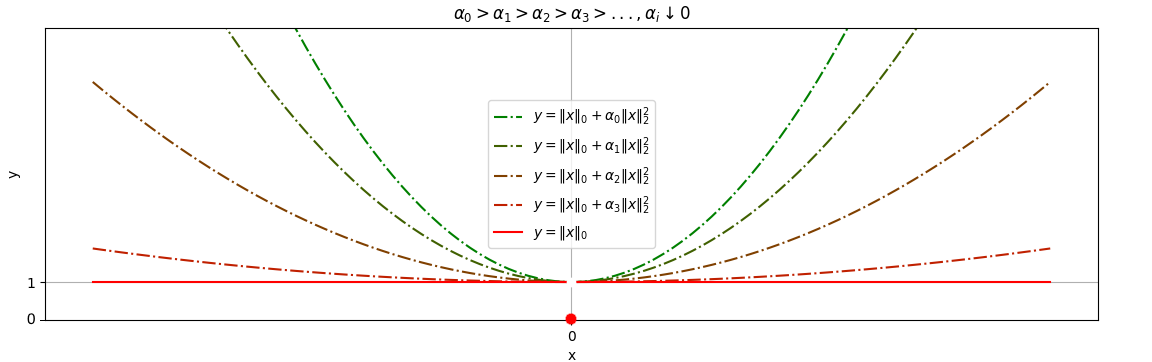
\includegraphics[width=0.9\textwidth]{l0l2towardsl0} % Resizes to 50% of text width
    \caption{$l_0l_2$ towards $l_0$.} % Adds a numbered caption
    \label{fig:l0l2towardsl0}        % Unique ID for cross-referencing
\end{figure}
    \section{Questions} % creates a section
\begin{itemize}
\item Is there cases where sparse modeling with $\left\|.\right\|_0 + \frac{1}{\delta^2} \left\|.\right\|_2^2$ is "better" or "more appropriate" than $\left\|.\right\|_0 $  solely? In what sense? Where?  When? How?
\item Is sparse modeling with $\left\|.\right\|_0 + \frac{1}{\delta^2} \left\|.\right\|_2^2$ more "tracktable" than $\left\|.\right\|_0$ from the point of view of mathematical programming?
\end{itemize}
\section*{References}
\begin{thebibliography}{99} % The '9' handles up to 9 references

\bibitem{Bertsimas2024}
Bertsimas, D., \& Johnson, N.A.G.:  \textit{Compressed sensing: a discrete optimization approach.} Mach Learn  (2024), 113, 6725–6764.

\bibitem{Lethi2016}
Le Thi, H. A. L., Pham Dinh, T., \& Thiao, M.: \textit{Efficient approaches for l2-l0 regularization
and applications to feature selection in SVM.} Applied Intelligence (2016), 45:549–565.

\bibitem{Soussen2013}
Soussen, C.: \textit{Algorithmes d'approximation parcimonieuse inspir\'es  d'Orthogonal Least Squares pour les probl\`emes inverses.} Traitement du signal et de l'image. Université de Lorraine, (2013).
\end{thebibliography}
\end{document} % This is the end of the document
